\documentclass[12pt]{beamer}
\usepackage{beamerthemeHannover, graphicx, clrscode, amsmath, amssymb, multicol}
\usepackage{textcomp} \usepackage{verbatim}
\usepackage{listings}
\setbeamercolor{sidebar}{use=structure,bg=red}

\author[@dukeleto]{Jonathan "Duke" Leto\\\small{@dukeleto\\letolabs.com\\duke@leto.net}}
\date{}
\title[Git.init()\hspace{2em}\insertframenumber/
\inserttotalframenumber]{Learning To Love The DAG For Fun And Profit}
\setbeamertemplate{navigation symbols}{} %no nav symbols

% keynote-ish
\renewcommand\sfdefault{phv}
\renewcommand\familydefault{\sfdefault}
\usetheme{default}
\usepackage{color}
\useoutertheme{default}
\usepackage{texnansi}
\usepackage{marvosym}
\definecolor{bottomcolour}{rgb}{0.32,0.3,0.38}
\definecolor{middlecolour}{rgb}{0.08,0.08,0.16}
\setbeamerfont{title}{size=\Huge}
\setbeamercolor{structure}{fg=gray}
\setbeamertemplate{frametitle}[default]%[center]
\setbeamercolor{normal text}{bg=black, fg=white}
\setbeamertemplate{background canvas}[vertical shading]
[bottom=bottomcolour, middle=middlecolour, top=black]
\setbeamertemplate{items}[circle]
\setbeamerfont{frametitle}{size=\huge}
\setbeamertemplate{navigation symbols}{} %no nav symbols

\begin{document}

\frame[t]{
    \begin{center}
            %
\includegraphics[scale=0.15]{pdxgit-simantel-green}
            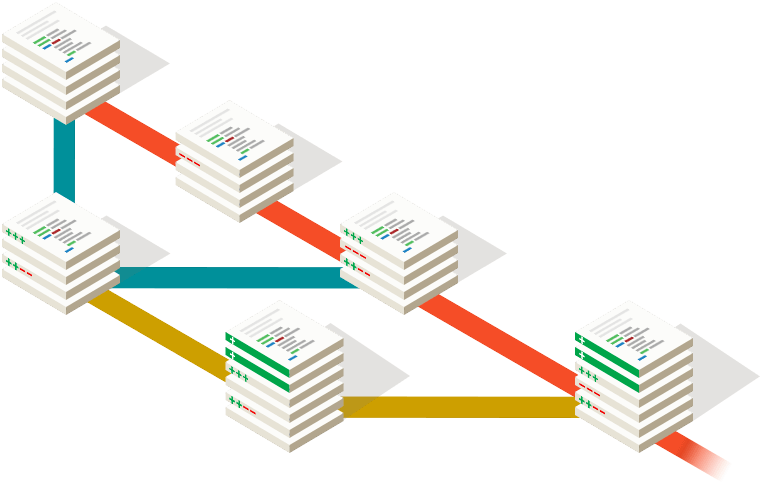
\includegraphics[scale=0.15]{branching}

    \end{center}
    \titlepage
}

\frame{
    \frametitle{Sponsors}
    \begin{center}
        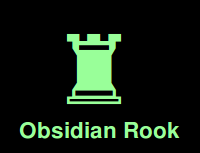
\includegraphics[scale=1]{unirook}
    \end{center}
}

\frame{
    \frametitle{Sponsors}
    \begin{center}
        
\includegraphics[scale=0.4]{shutterstock}
    \end{center}
}

\frame{
    \frametitle{Sponsors}
    \begin{center}
        
\includegraphics[scale=0.4]{geekdom}
    \end{center}
}

\frame{
    \frametitle{Sponsors}
    \begin{center}
        
\includegraphics[scale=0.5]{rackspace}
    \end{center}
}

\frame{
    \frametitle{ 
\includegraphics[scale=0.2]{pdxgit} A Bit About Me }
    \begin{center}
        \begin{itemize}
            \item PDX Git Together
            \item Git consulting
            \item Parrot Virtual Machine
            \item Google Summer of Code
            \item Google Code In
            \item BrewPony
            \item Mozillian
            \item ...
            \item Too many things
        \end{itemize}
    \end{center}
}

\frame{
    \frametitle{PDX Git Together }
    World's First Git User Group
    \begin{itemize}
        \item GSoC Mentor Summit Oct 2010
        \item Git Together Developer Conf Oct 2010
        \item GSoC Mentor Summit Oct 2011
        \item Git Together Developer Conf Oct 2011
        \item 26. Jan 2012 pdxgit.com
        \item 1. Feb 2012 1st Meeting
        \item 27. Aug 2012 2nd Meeting (@igalko)
        \item Now a regular monthly meeting!
    \end{itemize}
}

\frame{
    \frametitle{What *is* Git, exactly?}
    \begin{center}
        \begin{itemize}
        \item A DAG (Directed Acyclic Graph)
        \item A content tracker
        \item A diverse community with a common bond
        \item A collection of implementations
        \end{itemize}
    \end{center}
}

\frame{
    \frametitle{What *is* Git, exactly?}
    DAG = Directed Acyclic Graph
    \begin{center}
        \begin{itemize}
        \item a "Tree of Arrows"
        \item You can't be your own Grandpa
        \item Graph = nodes + vertices
        \end{itemize}
    \end{center}
}

\frame{
    \frametitle{What *is* Git, exactly?}
    A content tracker
    \begin{center}
        \begin{itemize}
        \item Originally "an information manager from hell"
        \item Track changes in content, storing the diffs
        \item An empty directory has no content
        \end{itemize}
    \end{center}
}

\frame{
    \frametitle{What *is* Git, exactly?}
    A diverse community with a common bond
    \begin{center}
        \begin{itemize}
        \item Started with Linus in kernel-land and then spread quickly
        \item Now: web app developers, UI designers, scientists, professors...
        \end{itemize}
    \end{center}
}

\frame{
    \frametitle{What *is* Git, exactly?}
    A Collection of Implementations
    \begin{center}
        \begin{itemize}
        \item "official" Git 1.x
        \item JGit - Git 1.x server in Java
        \item libgit2 - "fresh start" linkable library in C
        \item js-git - Very alpha implementation in Javascript
        \end{itemize}
    \end{center}
}


\frame{
    \frametitle{What *is* Git, exactly?}
    Git 1.x
    \begin{center}
        \begin{itemize}
        \item /bin/sh
        \item C
        \item Perl (git svn, git add -i)
        \item Some optional optimized assembly
        \end{itemize}
    \end{center}
}

\frame{
    \frametitle{What *is* Git, exactly?}
    JGit
    \begin{center}
        \begin{itemize}
        \item Git server written in Java
        \item Eclipse
        \item Gerrit Code Review
        \item various commercial products
        \end{itemize}
    \end{center}
}

\frame{
    \frametitle{What *is* Git, exactly?}
    libgit2.github.com
    \begin{center}
        \begin{itemize}
        \item No dependencies
        \item ANSI 89 C for max(portability)
        \item Linkable, re-entrant C library
        \item Designed for multi-threading
        \item Funded by: Github + Microsoft
        \end{itemize}
    \end{center}
}

\frame{
    \frametitle{Using libgit2 from Perl 5}

    \begin{center}
        \begin{itemize}
        \item use Git::Raw;
        \item Low-level access to Git objects
        \item Plumbing, not porcelain
        \end{itemize}

    
\includegraphics[scale=0.5]{cat-tube}

    \end{center}
}

\frame{
    \frametitle{What *is* Git, exactly?}
    Git::Raw example
    \lstinputlisting{git-raw-example.pl}
}

\frame{
    \frametitle{Using Git from Perl 5}
    use Git::Repository;
    \begin{center}
        \begin{itemize}
        \item Shells out to normal git binary
        \item Implements plumbing + porcelain
        \end{itemize}
    \end{center}
}

\frame{
    \frametitle{What *is* Git, exactly?}
    Git::Repository example
    \lstinputlisting{git-repo-example.pl}
}

\frame{
    \frametitle{What *is* Git, exactly?}
    github.com/creationix/js-git
    \begin{center}
        \begin{itemize}
        \item Git in Pure JavaScript
        \item Currently only read-only support
        \item Funded on bountysource.com
        \item Large donations from Mozilla + Adobe
        \end{itemize}
    \end{center}
}

\frame{
    \frametitle{Git + Perl community similarities}
    \begin{center}
        \begin{itemize}
        \item Perl 5 $\sim$ Git 1.x
        \item Perl 6 $\sim$ libgit2
        \end{itemize}
    \end{center}
}


\frame{
    \frametitle{Using Git}
    Git - The command line isn't the only way
    \begin{center}
        \begin{itemize}
        \item git gui
        \item Github for Mac/Windows
        \item GitX-dev
        \item Atalassian SourceTree
        \end{itemize}
    \end{center}
}

%\frame{
%    \frametitle{}
%    \begin{center}
%        \begin{itemize}
%        \item 
%        \end{itemize}
%    \end{center}
%}

\frame{
    \frametitle{Recent Features: 1.8.4}
    \begin{huge}
    git clean -i
    \end{huge}

    "interactive cleaning"
}
\frame{
    \frametitle{Useful Features}

    \begin{huge}
    git checkout -
    \end{huge}

    "checkout the last branch I was on"
}

\frame{
    \frametitle{Useful Features}

    \begin{huge}
    git merge -
    \end{huge}

    "merge the last branch I was on"
}

\frame{
    \frametitle{Useful Features}

    git blame -L 20,50 foo.txt \# lines 20-50

    git blame -L 10,+10 foo.txt \# lines 10-20

    git blame -L 50,-10 foo.txt \# lines 40-50
}

\frame{
    \frametitle{Coming Soon! in 1.8.5}

    git log HEAD <=> git log @
}
\frame{
    \frametitle{Coming Soon! in 1.8.5}

    git -C foo/ status $\sim$ make -C foo/
}

\frame{
    \frametitle{Interesting Git Use Case}
    The Open Tree of Life \\
    github.com/opentreeoflife
    \begin{center}
        \begin{itemize}
            \item Digital representation of the Tree Of Life
            \item Storing JSON files in Git
            \item Version control for evolution!
            \item Currently implementing a web API around Git repo
        \end{itemize}
    \end{center}
}

\frame{
    \frametitle{Extra Credit}
    \# Read the first Git commit by Linus himself

    \# Thu Apr 7 15:13:13 2005

    \$ git clone git://github.com/git/git.git

    \$ git show e83c5163
}

\frame{
    \frametitle{How I Can Help You}
    Git It Together
    \begin{center}
        \begin{itemize}
            \item Educating stakeholders on the value of Git
            \item On-site Training
            \item Implementing Git at your organization
            \begin{itemize}
                \item Converting from cvs|svn|? $\rightarrow$ Git
                \item Continuous Integration
                \item Deployment from Git
                \item Custom workflow creation + documentation
            \end{itemize}
            \item letolabs.com
        \end{itemize}
    \end{center}
}

\frame{
    \frametitle{git merge -s=social}
    \begin{center}
        \begin{itemize}
           \item @dukeleto
           \item 209.691.DUKE
           \item letolabs.com
           \item duke@leto.net
           \item linkedin.leto.net
           \item IRC: dukeleto on Freenode, Mozilla, Perl
        \end{itemize}
    \end{center}
}


\frame{
    \frametitle{Mahalo!}
    
\includegraphics[scale=1.5]{pdxgit}
    % 
\includegraphics[height=\paperheight]{pdxgit}
}
\end{document}
